\chapter{FEASIBILITY ANALYSIS OF THE POMDP OPTIMAL POLICY ON ESP$32$ RADIOS}\label{D}
In this chapter, we detail the implementation of the POMDP optimal spectrum sensing and access policy (from Chapter \ref{C}) on ad-hoc distributed network consisting of ESP32 radios, in order to prove the feasibility of our formulation. Section \ref{D.I} details the methodology followed in implementing the POMDP optimal sensing and access policy; Section \ref{D.II} describes the results obtained from this implementation; and Section \ref{D.III} involves concluding arguments.

\section{Methodology}\label{D.I}
We employ $8$ ESP32 radios \cite{Espressif:ESP32}, with each one embedded in a GCTronic e-puck2 robot \cite{GCTronic:epuck2}, categorized into a network of $3$ PUs (and their $3$ corresponding sinks) occupying $6$ channels in the discretized spectrum of interest according to a Markovian time-frequency correlation structure (described by \eqref{6})\texttt{-{}-}and $2$ independent SUs, with each having the capability of sensing only one channel at a time, intelligently trying to exploit the white-spaces in the spectrum. The detailed methodology of this implementation is provided below:
\begin{enumerate}
    \item Considering a network with $J{=}3$ PUs and one SU with a channel sensing restriction of $\kappa{=}2$ out of $K{=}6$ channels in the discretized spectrum of interest\texttt{-{}-}and assuming a linear AWGN observation model, with a Rayleigh channel fading model (discussed in Section \ref{I.I}), we simulate the occupancy behavior of the PUs according to a Markovian time-frequency correlation structure parameterized by $\vec{\theta}{=}[\vec{p},\vec{q}]^{\intercal}$, where $\vec{p}{=}[p_{00}{=}0.1,p_{01}{=}0.3,p_{10}{=}0.3,p_{11}{=}0.7]^{\intercal}$ and $\vec{q}{=}[q_{0}{=}0.3,q_{1}{=}0.8]^{\intercal}$; and solve for the optimal spectrum sensing and access policy using PERSEUS, embedded with a concurrent parameter estimation algorithm learning the parameter vector $\vec{\theta}$\texttt{-{}-}by mimicking the observational capabilities of the actual ESP32 radios. Note this step is performed on a PC.
    \item The simulated PU occupancy behavior\texttt{-{}-}Markovian correlated according to \eqref{6} and parameterized by $\vec{\theta}$, and the time-slot specific optimal channel access decisions (derived off of the POMDP optimal sensing policy and the simulated PU occupancy behavior), are stored in databases (for export onto the ESP32 network).
    \item Peer-to-Peer communication links are established between a PU ESP32 radio and its sink, using the $3$ ESP32 radios designated as PUs\texttt{-{}-}in other words, $3$ wireless communication links are established: one for each ESP32 PU pair (a source and a sink), over WiFi ($2.4$GHz) and using a channel according to the occupancy information detailed in the exported PU occupancy database, in time-slot $i$.
    \item Note here that in this ESP32 PU network implementation, in time-slot $i$, while establishing a wireless communication link between a ESP32 PU $j{\in}\{1,2,3\}$ and its respective sink $i{\in}\{1,2,3\}\text{ s.t.}i\text{ is the designated sink for PU}j$, i.e., while forming link $l_{ij}$ over channel $k_{l_{ij}}{=}k{\in}\{1,2,\dots,6\}$ (as determined by the exported PU occupancy database which contains simulated PU occupancy behavior according to the Markovian time-frequency correlation structure described above) such that $k_{l_{ij}}{\neq}k_{l_{i',j'}},{\forall}i,i'{\in}\{1,2,3\},j,j'{\in}\{1,2,3\}$\texttt{-{}-}PU $j$ serves as an Access Point (AP) accepting transmission requests from PU $i$, which is designates as a STAtion (STA). In the next synchronized time-slot $i+1$, this link $l_{ij}$ moves to channel $k'{\in}\{1,2,\dots,6\}$, as detailed in the exported PU occupancy database. This same procedure takes place for the other two incumbent communication links in every time-slot until the end of the implementation evaluation period.
    \item Although the PC-based POMDP solver employs an SU which can access $2$ channels at a time in order to deliver its flows (see the access part of the POMDP formulation in Section \ref{I.IV}), we employ $2$ ESP32 SU radios in the network\texttt{-{}-}with the channel access work synchronously and evenly split between the two\texttt{-{}-}due to the actual physical design limitation of the ESP32 radio that a it can only access one channel at a time, forcing us to be creative: split the optimal $2$ channel access decision in time-slot $i$, as determined by the time-slot specific optimal POMDP channel access database, into a single-channel access action at each ESP32 SU radio. Next, based on whether the channel access at the $2$ ESP32 SU radios was successful, we compute the success rate.
\end{enumerate}
\section{Implementation Results}\label{D.II}
The channel access success rate metric defined as
\begin{equation}\label{C.I}
    \text{Channel Access Success Probability}=\frac{\sum_{j=1}^{2}\mathcal{I}\left\{B_{k_{SU_{j}}}(i)=0\right\}}{2},
\end{equation}
where $\mathcal{I}$ corresponding to $\mathcal{I}\left\{B_{k_{SU_{j}}}(i)=0\right\}$ is an indicator variable whose value is $1$ if the channel accessed by the ESP32 SU $j{\in}\{1,2\}$ in time-slot $i$ is not occupied by an incumbent PU ESP32 radio, and $B_{k_{SU_{j}}}{\in}\{0,1\}$ is the occupancy variable of the channel accessed by the ESP32 SU $j$ in time-slot $i$\texttt{-{}-}is evaluated per time-slot $i$, and the resultant metrics are plotted against time, which is illustrated in Fig. \ref{fig:C.1}.
\begin{figure} [htb]
    \centerline{
    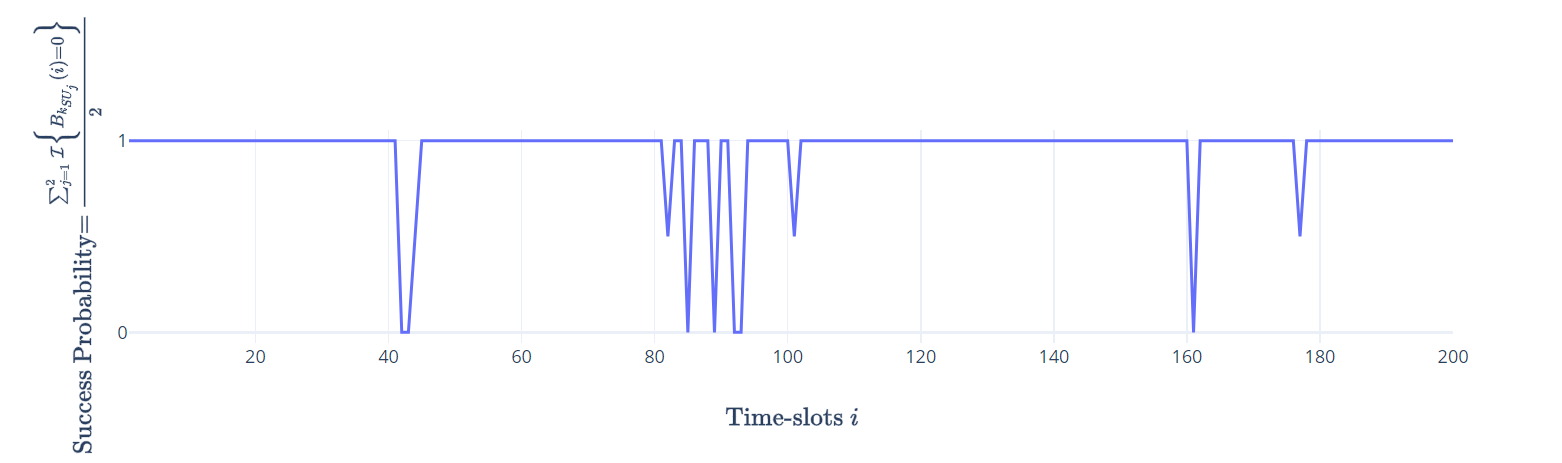
\includegraphics[width = 1.0\textwidth]{ESP32_Success_Probability.PNG}}
    \caption{The channel access probability of the ESP32 SU radios per time-slot}
    \label{fig:C.1}
\end{figure}
\section{Conclusion}\label{D.III}
In this chapter, we simulated an ad-hoc distributed peer-to-peer network with incumbent radios occupying the spectrum according to a Markovian time-frequency correlation structure, and an SU constituting a parameter estimator and a POMDP agent solving for the optimal channel sensing and access policy\texttt{-{}-}the simulated time-slotted incumbent occupancy behavior is exported onto a peer-to-peer network formed by actual ESP32 radios serving as PUs; and the time-slotted optimal channel access decisions are exported onto a peer-to-peer network formed by actual ESP32 radios serving as SUs (we use $2$ SUs in the actual implementation due to design limitations, with the access work split between the two, and merged upon completion). Upon merging the channel access results from both the ESP32 SU radios, we plot the SU network's success probability (given by \eqref{C.I})\texttt{-{}-}we find that the channel access decisions made by our SU network are accurate for a significant portion of the implementation evaluation period. The primary intention behind this analysis is to show that the optimal policy obtained by the POMDP solver with respect to an ad-hoc emulated network can be transferred (i.e., exported) onto the actual physical network with ease, by leveraging synchronization and data aggregation techniques.